\documentclass[10pt,oneside]{memoir}
\usepackage{listings}
\usepackage[utf8]{inputenc}
\usepackage{geometry}
\geometry{letterpaper}
\usepackage{graphicx,floatflt,wrapfig}
\usepackage{amssymb,amsmath,amsfonts,amsthm,accents}
\usepackage{empheq}
\usepackage{color}
\usepackage{url}
%\usepackage[notref,notcite]{showkeys}
\usepackage[pdftex,
            pdfauthor={Blaise Bourdin},
            pdftitle={vDef manual},
            pdfcreator={pdflatex},
            bookmarks=true,         % show bookmarks bar?
            unicode=false,          % non-Latin characters in Acrobat?s bookmarks
            pdftoolbar=true,        % show Acrobat?s toolbar?
            pdfmenubar=true,        % show Acrobat?s menu?
            pdffitwindow=false,     % window fit to page when opened
            pdfstartview={FitH},    % fits the width of the page to the window
            pdfnewwindow=true,      % links in new window
            colorlinks=true,
            linkcolor=blue,         % color of internal links
            citecolor=blue,         % color of links to bibliography
            filecolor=blue,         % color of file links
            urlcolor=blue,
            pagebackref=false,
            hyperfootnotes=true]{hyperref}
\usepackage{paralist}
\usepackage{verbatim}
\usepackage{algorithm,algpseudocode}


\def\vDef{{\texttt{vDef}} }
\DeclareMathOperator*{\argmin}{argmin}
\DeclareMathOperator{\e}{{\mathbf e}}

\title{\vDef user manual}
\author{Blaise Bourdin}
\date{\today}

\chapterstyle{section}
\begin{document}
\bibliographystyle{alpha}
\maketitle

\tableofcontents
\chapter*{Introduction}
\vDef is a reference implementation of the Variational Approach to Fracture~\cite{Francfort-Marigo-1998,Bourdin-Francfort-EtAl-2008b} and related problems. 


This brief manual lists the main command line options for \vDef with default values are shown between angled brackets \verb+<>+. Note that auto--generated documentation can always be printed using the \texttt{-h} and  \texttt{-verbose 1} flags, possibly combined with \texttt{-dryrun}.


\vDef uses the exodusII file format for its input and output. XDMF / HDF5--based export for very large data files is a planned feature but not available yet. Geometric entities corresponding to different materials, models or boundary conditions can be encoded using exodus ``element blocks'' (cell sets in \vDef lingo) and ``node sets'' (referred to as vertex sets). Note that exodusII ``side sets'' are not supported. Instead, \vDef uses cell sets of co-dimension 1.


\newpage
\chapter{Models and algorithms}
\section{Heat transfer}
\label{sec:HeatXfer}
\vDef can solve diffusive linear steady-state or transient heat transfer problems. This heat transfer solver can be used as a standalone simulator, or the temperature field can be plugged in the elasticity of gradient damage simulators. In the sequel, we consider the problem of finding the temperature $T(x,t)$ of a body occupying a region $\Omega$ of the two or three--dimensional space and satisfying
\begin{empheq}[left=\empheqlbrace]{align}
	\rho(x) c_p(x) \frac{\partial T}{\partial t} &= \mathrm{div}\left( K(x) \nabla T\right) + f & \text{ in } \Omega,\\
    K \frac{\partial T}{\partial n} (x,t)& = g(x,t) + H (T_e-T(x,t)) & \text{ on } \partial_n \Omega,\\
    T(x,t) & = T_b(x,t) & \text{ on } \partial_d \Omega,\\
    T(x,0) & = T_0. 
\end{empheq}
Where $f$ and $g$ denotes respectively the body and boundary fluxes, $T_b$ is a prescribed boundary temperature, $T_e$ is a constant surrounding temperature, and $T_0$ is a constant initial temperature. $\rho$ is the material's density, $c_p$ its specific heat, $K$ is the thermal conductivity, a symmetric tensor, and $H$ is the surface thermal conductivity. For steady state problems, time derivatives are ignored and the initial temperature is used as the initial guess of the iterative solver.


\section{Gradient damage models}
\label{sec:GradientDamageModels}
The damage models implemented in \vDef are regularization of the energy functional devised in the the variational approach to fracture~\cite{Ambrosio-Tortorelli-1990,Ambrosio-Tortorelli-1992,Giacomini-2005,Sicsic-Marigo-2013a}. These problems are formulated as rate independent unilateral minimization problems of a total energy functional
\begin{equation}
	\label{eq:defEll}
	\mathcal{E}_\ell(u,\alpha) := \int_\Omega s(\alpha) W(\e(u),T,\e^p)\, dx - \int_\Omega f\cdot u \, dx - \int_{\partial_n \Omega} \tau \cdot u \, ds + \frac{k}{4c_w} \int_\Omega \frac{w(\alpha}{\ell} + \ell|\nabla \alpha|^2\, dx,
\end{equation}
where $u$, and $\alpha$ denote the displacement and damage fields, $T$, $f$, $\tau$, and $\e^p$ are given temperature, body force, surface force and plastic deformation, $\ell$ is the material internal length, $W$ is linear elastic potential:
$$
W(\e,T,\e^p) := \frac{1}{2} \mathbf{A}\left(\e-T \alpha_L-\e^p\right):\left(\e-T \alpha_L-\e^p\right).
$$
$\mathbf{A}$ is the material's Hooke's law, $\alpha_L$ its linear thermal expansion tensor (a symmatric matrix).
The function $w$ is related to the energy dissipation function associated with a distributed damage field and the constant $c_w:= \int_0^1 \sqrt{w(s)}\, ds$ is a normalization constant.
Two variants are implemented ($\eta$ being a small \emph{residual stiffness} possibly set to 0):
\begin{itemize}
\item
	``AT1'': $s(\alpha) = \eta + (1-\alpha)^2$, $w(\alpha) = \alpha$, and $c_w =2/3$.
	``AT2'': $s(\alpha) = \eta + (1-\alpha)^2$, $w(\alpha) = \alpha^2$, and $c_w = 1/2$.
\end{itemize}
For a comparison of the properties, refer to~\cite{Pham-Amor-EtAl-2011a}.


 In the time discrete formulation, the displacement and damage field at time step $t_i$ are given by
\begin{equation}
	\label{eq:globMin}
	(u_i,\alpha_i) = \argmin_{v \in \mathcal{K}(t_i), \beta \in \mathcal{K}'(\alpha_{i-1},\eta)} \mathcal{E}_\ell(v,\beta),
\end{equation}
where $\mathcal{K}(t_i)$ is the set of kinematically admissible displacement fields at step $t_i$, and $\mathcal{K}'(\alpha_{i-1},\eta)$ is the set of all damage field satisfying the irreversibility condition
$$
	\mathcal{K}'(\alpha_{i-1},\eta) = \left\{\alpha \ :\  0 \le \alpha(x) \ge \alpha_{i-1}(x) \le 1 \ \forall x \text{ such that } \alpha_{i-1}(x) \ge \eta\right\}.
$$
Note that with these notations, enforcing irreversibility through inequality constraints as proposed in~\cite{Giacomini-2005,Amor-Marigo-EtAl-2008a,Pham-Amor-EtAl-2011a} corresponds to $\eta = 0$ whereas equality constraints under a threshold as originally proposed in~\cite{Bourdin-Francfort-EtAl-2000a} corresponds to $\eta$ close to 1.

\section{Backtracking algorithms}
\label{sec:BT}
Backtracking algorithms are based on enforcing necessary conditions for optimality for the entire time evolution~\cite{Bourdin-2007a}. They are based on a comparison principle: at each step, a test field admissible for all previous times is built and its energy compared to that of the previously computed ones. If the test field is of lesser energy that the previously computed one, the algorithm backtracks to this step and the alternate minimizations are restarted from the newly constructed test field. A standard and a \emph{deep} backtracking are implemented:

\begin{algorithm}
	\caption{Standard backtracking algorithm}
	\label{algo:StdBT}
		\begin{algorithmic}[1]
			\State Given N, $t_0 < t_1 < \dots < t_N$, $\mathrm{BT}_{tol}$:
			\State $i \leftarrow 0$
			\Repeat
				\State Compute $(u_i,\alpha_i)$ using alternate minimizations\label{altmin}
				\For{$j = i-\mathrm{BT}_{scope} \text{ to } i-1$}
					\If {$\frac{{t_j}^2}{{t_i}^2}\mathcal{U}_{t_j}(u_{t_i},\Gamma_{t_i}) + \mathcal{S}(\Gamma_t) \le \mathcal{U}_{t_j}(u_{t_j},\Gamma_{t_j}) + \mathcal{S}(\Gamma_{t_j}) - \mathrm{BT}_{tol}$}
						\State $i \leftarrow j$
						\State goto~\ref{altmin}
					\EndIf	
				\EndFor
				
			\Until{$i = n$}
			\State $i \leftarrow i+1$
		\end{algorithmic}
\end{algorithm}

In the deep backtracking, the exploration loop (lines 5-10) is moved into the alternate minimizations loop and executed every \verb+BT_Iinterval+ iterations. In addition, the exploration loop can be run forward (\verb+BT_Type Forward+) or backward (\verb+BT_Type Backward+).

\section{General limitations.}
\begin{itemize}
\item \vDef is based on PETSc-3.3~\cite{petsc-efficient,petsc-user-ref,petsc-web-page}. Unstructured meshes are handled using \texttt{Sieve}~\cite{Knepley-Karpeev-2009a}. A new version based on PETSc' \texttt{DMcomplex} is under development. PETSc-specific options are not described in this manual.
\item \vDef only supports the \href{http://sourceforge.net/projects/exodusii/}{exodusII} file format. \href{http://cubit.sandia.gov}{Cubit}, or \href{http://www.csimsoft.com/trelis.jsp}{Trelis} can generate such files. \href{https://wci.llnl.gov/codes/visit/}{VisIt}, \href{http://paraview.org}{ParaView}, or \href{http://www.ceisoftware.com}{EnSight} can open such files.
\item \vDef can handle linear and quadratic simplicial finite elements. Due to limitations of the exodus file formal, mixing element types is not supported at this point.
\item \vDef can import element blocks of co-dimension 0 and 1, and node sets. \emph{Node sets may not overlap}.
\item Boundary conditions can be specified on cell or vertex sets. Passing boundary conditions on vertex sets is slightly more efficient, but ensuring that vertex sets are disjoint can be difficult.
\item Boundary condition handling is \emph{additive}. If a cell or vertex belong to several sets, the type of boundary conditions is given by performing a logical \verb+OR+ on the boundary conditions type of its parent entities. 
%\item may lead to inconsistent results. In general, the loading applied will be the one specified in the set written last in the exodus file. There may be boundary effects for parallel computations.
%\item Work constrained evolution, multiple load sets, variational plasticity, thermodynamically consistent evolutions are not implemented in this version of vDef.
\end{itemize}

\chapter{Command line options}


\section{Options strings vs. YAML files}
Command line options can also be passed to vDef through an option file, using the \verb+-options_file+ command line flag. Machine readable \href{http://www.yaml.org}{YAML} files can be used with the flag \verb+-options_file_yaml+. YAML parsing is fragile, incomplete, and somewhat experimental (alias and links are not implemented, and error reporting is lacking), but much easier to parse. PETSc  uses  underscores as field delimiters in its options handling and keeps track of hierarchy of options through prefixes, Whereas YAML relies on indented lists. The correspondence between standard options and YAML file straightforward, with a few caveats: array arguments must be given as space delimited in PETSc options but comma delimited without spaces in YAML and boolean arguments can be given the value \verb+0,false,no+ or \verb+1,true,yes+ in PETSc but only \verb+0,no+ or \verb+1,yes+ are acceptable in a YAML option file. An example of translation from PETSC--like to YAML options is given in Table~\ref{tab:PETSctoYAML}.

\begin{table}
PETSc--like options string\\
\small{
\begin{boxedverbatim}
-time_min 0 -time_max 1 -time_interpolation linear -time_numstep 11  -dryrun \
-cs0001_hookeslaw 1. 0. 0. .5 0. 1. -cs0001_fractureToughness .1 \
-cs0001_internalLength 01 -cs0001_residualStiffness 0.\
-cs0001_defectLaw_type gradientDamage \
-cs0001_defectLaw_gradientDamage_type AT1 \
-cs0001_displacementBC true false false -cs0001_boundaryDisplacement 1. 0. 0. \
-cs0001_damageBC false
\end{boxedverbatim}
}
Equivalent YAML file\\
\small{
\begin{boxedverbatim}
time:
    min: 0
    max: 1
    interpolation: linear
    numstep: 11
cs0001:
    HookesLaw: 1.,0.,0.,.5,0.,1.
    fractureToughness: .1
    internalLength: .1
    residualStiffness: 0.
    defectLaw:
        type: GradientDamage
        gradientDamage:
            type: AT1
    displacementBC: yes,no,no
    boundaryDisplacement: 1.,0.,0.
    damageBC: no
\end{boxedverbatim}
}
\caption{Translating PETSc options to YAML files}
\label{tab:PETSctoYAML}
\end{table}

\section{General options}
\begin{boxedverbatim}
-prefix : File name prefix
-verbose <1>: Verbosity: level 
-dryrun <FALSE>: Dry run in order to validate the options file. 
-file_format <EXOSingle>: (MEF90FileFormat) I/O: file format. 
                          Choose one of EXOSingle EXOSplit
\end{boxedverbatim}
Notes: 
\begin{compactenum}
\item File names are not user configurable. \vDef will look for an input mesh is named \verb+<prefix>.gen+, results will be saved as \verb+<prefix>_out.gen+ or \verb+<prefix>-\%4i.gen+ if output in split files exodus files is chosen), energies will be saved in  \verb+<prefix>.ener+ for the entire domain and \verb+<prefix>-\%4i.enerblk+ for each cell set.
\item If \verb+ -file_format EXOSplit+ is selected (not recommended), each core will save its own part of the geometry in a separate file. Continuity at the subdomain interfaces is not preserved (no ghost points or interface matching informations are saved).
\end{compactenum}

\subsection{Ordering of tensors}
In all options, symmetric tensors or order 2 (symmetric matrices) are given in Voigt notations, \emph{i.e.} a $3\times 3$ symmetric matrix is represented by the array $A_{11},A_{22},A_{33},A_{23},A_{13},A_{12}$ and a $2\times 2$ symmetric matrix as $A_{11},A_{22},A_{12}$. 
The symmetric fourth order tensors (Hooke's laws) are stored as the rows of the upper diagonal part of a matrix consistent with the ordering above, i.e.
\begin{equation*}
	\begin{bmatrix}
		C_{1111} & C_{1122} & C_{1133} & C_{1123} & C_{1113} & C_{1112}\\
				 & C_{2222} & C_{2233} & C_{2223} & C_{2213} & C_{2212}\\
				 &          & C_{3333} & C_{3323} & C_{3313} & C_{3312}\\
				 &          &          & C_{2323} & C_{2313} & C_{2312}\\
				 &          &          &          & C_{1313} & C_{1312}\\
				 &          &          &          &          & C_{1313}
	\end{bmatrix}
\end{equation*}
becomes:
$\left[C_{1111}\ C_{1122}\  C_{1133}\  C_{1123}\  C_{1113}\  C_{1112}\  C_{2222}\  \dots  C_{1312}\  C_{1313}\right]$.

A small utility in \verb+$MEF90_DIR/Tests/HookeLaws+ can be used to compute the coefficients of isotropic Hooke's laws:
\begin{boxedverbatim}
bourdin@galerkin:Tests $ ./HookeLaws -E 1 -nu .3
 # MEF90: hg changeset 1792:b88429f29d30 
 # Copyright (c) 1998-2014 B. Bourdin <bourdin@lsu.edu> 
 # PETSC_ARCH=Darwin-gcc5.0-mef90-g 
 # PETSC_DIR=/opt/HPC/petsc-3.3-p7 
  
Hooke's laws for E= 1.00E+00 nu= 3.00E-01
 3D isotropic
 1.34615E+00, 5.76923E-01, 5.76923E-01, 0.00000E+00, 0.00000E+00, 0.00000E+00, 
 1.34615E+00, 5.76923E-01, 0.00000E+00, 0.00000E+00, 0.00000E+00, 1.34615E+00, 
 0.00000E+00, 0.00000E+00, 0.00000E+00, 3.84615E-01, 0.00000E+00, 0.00000E+00, 
 3.84615E-01, 0.00000E+00, 3.84615E-01 
 2D plane stress
 1.09890E+00, 3.29670E-01, 0.00000E+00, 1.09890E+00, 0.00000E+00, 3.84615E-01 
 2D plane strain
 1.34615E+00, 5.76923E-01, 0.00000E+00, 1.34615E+00, 0.00000E+00, 3.84615E-01 
\end{boxedverbatim}

Alternatively, \emph{isotropic} Hooke's laws are also implemented (see Section~\ref{sec:MatProp}).


\subsection{Time interpolation}
\small{
\begin{boxedverbatim}
-time_min <0>: Time: min 
-time_max <1>: Time: max 
-time_numstep <11>: Time: number of time steps 
-time_interpolation <linear>: Time: interpolation type. One of linear quadratic exo
\end{boxedverbatim}
}
Notes: 
\begin{compactenum}
	\item If \verb+-time_interpolation exo+ is selected, analysis times will be loaded from the \emph{output} exodus file, which is expected to exist.
	\item \verb+-time_interpolation quadratic+ corresponds to the natural time scaling in many heat transfer problems, i.e. $\tau$ is linearly interpolated between $\sqrt{t_{min}}$ and $\sqrt{t_{max}}$, and $t_i = \tau_i^2$.
\end{compactenum}

\subsection{Offset and scaling}
It is possible to specify the order in which fields in an exodus file are saved by specifying and \emph{offset}. An offset of 0 can be used to indicate that a specific field is not to be saved in the file.

Piecewise constant loadings functions (fluxes, forces, boundary values) can be passed through the command line. Their time dependence can be controlled using the keywords \verb+constant+, \verb+linear+, or \verb+null+. When the scaling is set to null, \vDef will skip assembly of the field, when possible. The \verb+EXO+ keyword is used to indicate that the values are to be read from the \emph{output} file.

\section{Problem description}
Due to a bug in the ExodusII fortran bindings, \vDef can only import Exodus entities numbers and ignores their names. When passing command line options, Exodus' element blocks are abbreviated as \verb+cs+ (for Cell Sets) and nodes sets as \verb+vs+ (for Vertex Sets) concatenated with the entity number formatted with 4 digits. For instance, the prefix associated with exodusII element block 10 would be \verb+cs0010_+.

\subsection{Material properties}
\label{sec:MatProp}
Material properties for a cell set are passed by prefixing the following options with the cell set number (i.e. \verb+-cs0001_Density+, for instance). Materials names are not used at the moment. Substitute the \verb+cs0001_+ prefix with the appropriate reference.
\small{
\begin{boxedverbatim}
-cs0001_Name <MEF90Mathium2D>:  
-cs0001_Density <1>: [kg.m^(-2)] (rho) Density 
-cs0001_FractureToughness <1>: [N.m^(-1)] (G_c) Fracture toughness 
-cs0001_SpecificHeat <1>: [J.kg^(-1).K^(-1)] (Cp) Specific heat 
-cs0001_ThermalConductivity <1 1 0 >: [J.m^(-1).s^(-1).K^(-1)] (K) Thermal conductivity 
-cs0001_LinearThermalExpansion <1 1 0 >: [K^(-1)] (alpha) Linear thermal expansion  
-cs0001_HookesLaw <1 0 0 .5 0 1 >: [N.m^(-2)] (A) Hooke's law 
-cs0001_internalLength <1>: [m] (l) Internal Length 
\end{boxedverbatim}
}

Isotropic Hookes laws are described in terms of  Youngs Modulus / Poisson ration in plane stress or plane strain (2D only) as:
\begin{boxedverbatim}
-cs0001_hookeslaw_type = Isotropic; (MEF90HookesLawTypeList) Type of Hooke's law
-cs0001_hookeslaw_YoungsModulus = 1 ; [N.m^(-2)] (E) Young's Modulus
-cs0001_hookeslaw_PoissonRatio = 0.3 ; [] (nu) Poisson Modulus
-cs0001_hookeslaw_planeStress =  FALSE; Use plane stress elasticity
\end{boxedverbatim}
or as a general fourth order tensor.

\subsection{Heat transfer options}
\subsubsection{Global options}
\small{\begin{boxedverbatim}
-heatxfer_mode <SteadyState>:   Type of heat transfer computation 
                                choose one of null SteadyState Transient
-heatxfer_addNullSpace <FALSE>: Add null space to SNES 
-temp_Offset <1>:               Position of temperature field in EXO file 
-heatxfer_initialTemp <0>:      [K] (T): Initial Temperature 
-boundaryTemp_scaling <linear>: Boundary temperature scaling 
                                choose one of)  constant linear file null
-boundaryTemp_Offset <0>:       Position of boundary temperature field in EXO file 
-externalTemp_scaling <linear>: External Temperature scaling 
                                choose one of constant linear file null
-externalTemp_Offset <2>:       Position of external temperature field in EXO file 
-flux_scaling <linear>:         Heat flux scaling 
                                choose one of constant linear file null
-flux_Offset <1>:               Position of heat flux field in EXO file 
\end{boxedverbatim}}

\subsubsection{Cell sets options}
\small{\begin{boxedverbatim}
-cs0001_ShortID <1>: Element type ShortID 
-cs0001_Flux <0>: [J.s^(-1).m^(-3) / J.s^(-1).m^(-2)] (f): Body / surface heat flux 
-cs0001_SurfaceThermalConductivity <0>: [J.s^(-2).m^(-1).K^(-1)]
                                        (H) Surface Thermal Conductivity 
-cs0001_externalTemp <0>: Surrounding temperature T [K] 
-cs0001_TempBC <FALSE>:   Temperature has Dirichlet boundary Condition (Y/N) 
-cs0001_boundaryTemp <0>: Temperature boundary value 
\end{boxedverbatim}}
Notes:
\begin{compactenum}
\item Element shortID should not be changed manually. 
\item Surrounding temperature is assumed to be constant. This could easily be changed.
\end{compactenum}

\subsubsection{Vertex sets options}
\small{\begin{boxedverbatim}
-vs0500_TempBC <FALSE>:   Temperature has Dirichlet boundary Condition (Y/N) 
-vs0500_boundaryTemp <0>: Temperature boundary value 
\end{boxedverbatim}}

\subsection{Gradient damage options}
\subsubsection{Global options}
\small{\begin{boxedverbatim}
-DefMech_mode <QuasiStatic>: Type of defect mechanics computation. 
                             Choose one of Null QuasiStatic GradientFlow
-disp_addNullSpace <TRUE>: Add null space to SNES 
-displacement_Offset <3>: Position of displacement field in EXO file 
-damage_Offset <2>: Position of damage field in EXO file 
-boundaryDamage_Offset <0>: Position of boundary damage field in EXO file 
-stress_Offset <6>: Position of stress field in EXO file 
-temperature_Offset <1>: Position of temperature field in EXO file 
-plasticStrain_Offset <0>: Position of the plastic Strain field in EXO file 
-boundaryDisplacement_scaling <linear>: Boundary displacement scaling.
                                        Choose one of constant linear file null
-boundaryDisplacement_Offset <3>: Position of boundary displacement field in EXO file 
-boundaryDamage_scaling <constant>: Boundary damage scaling.
                                    Choose one of constant linear file null
-force_scaling <linear>: Force scaling. 
                         Choose one of constant linear file null
-force_Offset <4>: Position of force field in EXO file 
-pressureForce_scaling <linear>: Pressure force scaling. 
                                 Choose one of constant linear file null
-pressureForce_Offset <3>: Position of pressure force field in EXO file 

-defmech_damage_atol <0.0001>: Absolute tolerance on damage error 
-defmech_maxit <1000>: Maximum number of alternate minimizations for damage 
-defmech_irrevThres <0>: Threshold above which irreversibility is enforced 
                        (0 for monotonicity, .99 for equality) 

-BT_Type <Null>: Backtracking type.
                 Choose one of Null Backward Forward
-BT_Interval <-1>: Interval at which Backtracking is run in inner loop 
                   (<0 for outer loop) 
-BT_Scope <-1>: Backtracking scope (<0 for unlimited) 
-BT_Tol <0.01>: Backtracking relative tolerance 
\end{boxedverbatim}}
Notes:
\begin{compactenum}
\item Element shortID should not be changed manually. 
\item \verb+-BT_Interval 1+ is for \emph{deep} backtracking, \verb+-BT_Interval -1+ for a standard backtracking.
\end{compactenum}

\subsubsection{Cell sets options}
\small{\begin{boxedverbatim}
-cs0001_ShortIDDisplacement <3>: Displacement element type ShortID 
-cs0001_ShortIDDamage <1>: Damage field element type ShortID 
-cs0001_Force <0 1 2 >: [N.m^(-3) / N.m^(-2) / N.m^(-1)] (f): body / boundary force 
-cs0001_pressureForce <0>: [N.m^(-2) / N.m^(-1)] (p): boundary pressure force 
-cs0001_defectLaw_type <GradientDamage>: Type of defect law. Choose one of 
                                         Elasticity GradientDamage Plasticity
-cs0001_defectLaw_gradientDamage_type <AT1>: Ambrosio-Tortorelli variant. 
                                             Choose one of AT1 AT2
-cs0001_DisplacementBC <0 1 2 >: Displacement has Dirichlet boundary Condition (Y/N) 
-cs0001_boundaryDisplacement <0 1 2 >: [m] (U): Displacement boundary value 
-cs0001_DamageBC <FALSE>: Damage has Dirichlet boundary Condition (Y/N) 
-cs0001_boundaryDamage <0>: [unit-less] (alpha): Damage boundary value 
-cs0001_residualStiffness <1e-09>: [unit-less] (eta): residual stiffness multiplier 
\end{boxedverbatim}}
Notes:
\begin{compactenum}
\item Element shortID should not be changed manually.
\item \verb+defectLaw+ and children have no effect on cell sets of codimension 1
\item \verb+defectLaw_type plasticity+ is not implemented right now.
\item \verb+defectLaw+, (and fracture toughness and internal length) must be given even when \verb+defectLaw_type elasticity+ is used. See Section~\ref{sec:GradientDamageModels} for details
\end{compactenum}


\subsubsection{Vertex sets options}
\small{\begin{boxedverbatim}
-vs0500_DisplacementBC <0 1 2 >: Displacement has Dirichlet boundary Condition (Y/N) 
-vs0500_boundaryDisplacement <0 1 2 >: [m] (U): Displacement boundary value 
-vs0500_DamageBC <FALSE>: Damage has Dirichlet boundary Condition (Y/N) 
-vs0500_boundaryDamage <0>: [unit-less] (alpha): boundaryDamage 
\end{boxedverbatim}}



\chapter{Examples}
\section{Uniaxial tension}
This example is studied in depth in~\cite[Section 3.1]{Bourdin-Francfort-EtAl-2008b} in the Griffith setting and in~\cite{Pham-Amor-EtAl-2011a} for gradient damage models.


We consider a rectangular domain $\Omega = (-L/2,L/2) \times (-H/2,H/2)$ subject to a monotonically increasing uniaxial displacement or surface force on its lateral edges. 


\begin{figure}[H]
\centering
	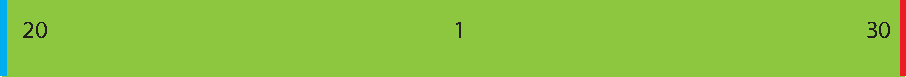
\includegraphics[width = \textwidth]{Examples/UniaxialTension/Geometry.pdf}
\caption{Domain for the uniaxial tension example. The numbers correspond to cubit entities.}
\label{fig:Uniaxial}
\end{figure}

Trelis journal files for this problem are located in \verb+Examples/UniaxialTension/UniaxialTension2D.jou+ and \verb+Examples/UniaxialTension/UniaxialTension3D.jou+. A sample YAML option file is located at \verb+Examples/UniaxialTension/UniaxialTension.yaml+

\section*{Proposed numerical experimentations:}
\begin{enumerate}
	\item	Using \verb+defectLaw_type AT1+ and \verb+defectLaw_type AT1+, study the interaction between mesh size and regularization length. For a given mesh, see how the surface energy depends on $\ell$. Check that this dependency can be avoiding by using an effective fracture toughness.
	\item Notice that the numerical solution without backtracking does not satisfy energy continuity and cannot be a global minimizer. Use a backtracking algorithm to compute a global minimizer.
	\item Without backtracking, see how the loading upon which crack nucleate depends on $\ell$.
	\item See how force driven computations will fail as soon as a critical force is reached.
	\item Compare algorithmic complexity, parallel performances of linear and quadratic finite elements for this problem.
\end{enumerate}

\section{Double Cantilever Beam}
It is well known that crack propagation in a standard shaped double cantilever beam sample is not stable. We consider a tapered geometry as shown in Figure~\ref{fig:DCB}. Various Trelis journal files for this problem are located in \verb+Examples/DCB+. For $L_1=1.25$, $L_2 = 4$, $L_3=1$, $R = .25$, $H_1=1$, $H_2 = 2$, a mesh size $h=.05$ will give approximately 25,0000 elements. A fracture toughness of $k=.01$ will lead to crack propagation when $0 \le t \le 1$.

\begin{figure}[H]
\centering
	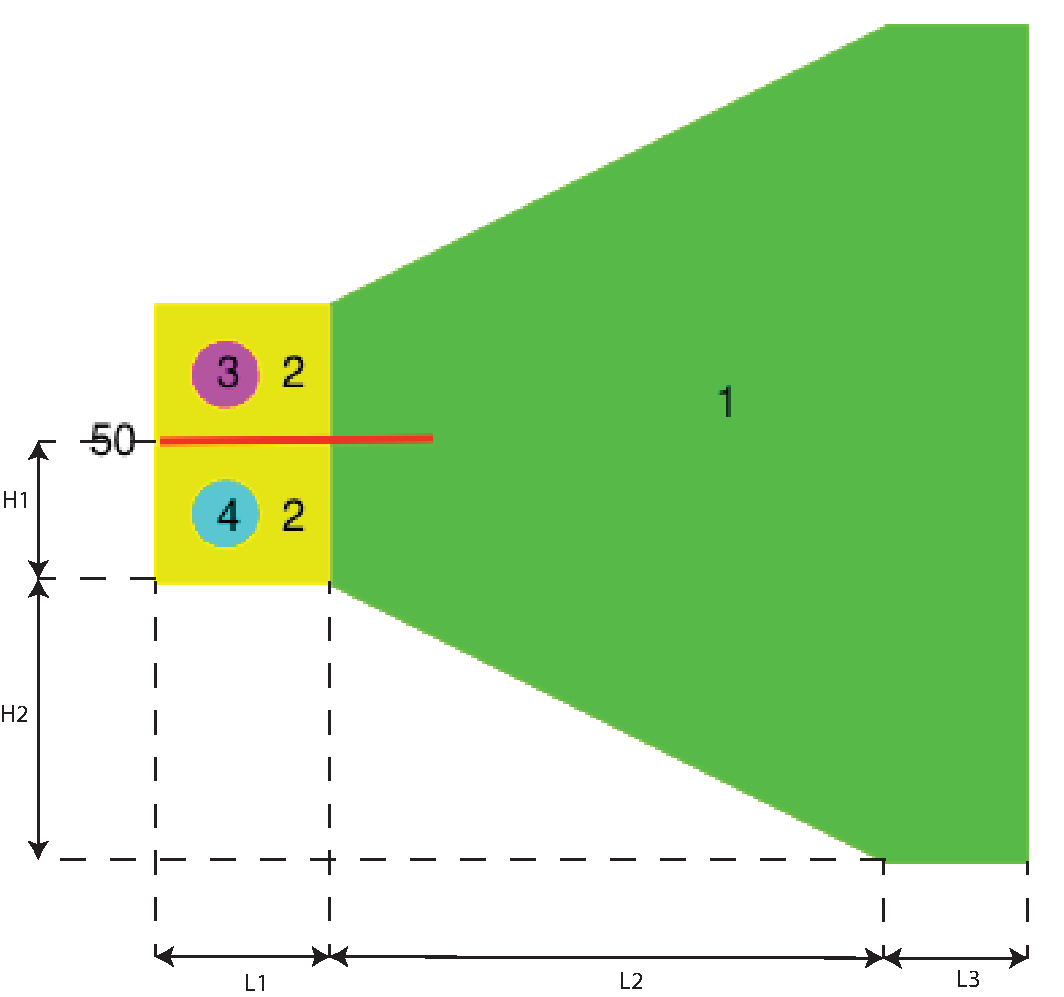
\includegraphics[width = .5\textwidth]{Examples/DCB/Geometry.pdf}
\caption{Domain for the DCB example. The numbers correspond to cubit entities.}
\label{fig:DCB}
\end{figure}

\section*{Proposed numerical experimentations:}
\begin{itemize}
	\item Prescribe the $y$ component of the displacement in cell sets 3 and 4. A symmetry argument could be used to infer that propagation will take place along the symmetry axis. Is this the case? 
	\item Fix both components of the displacement field on cell sets 3 and 4. 
	\item Add an inclusion in the crack path. See how varying the toughness and stiffness of the inclusion will either capture or divert the propagating crack.
\end{itemize}


\section{Surfing}
We consider a rectangular domain occupying a domain $\Omega = [\L/2,L/2] \times [-H/2,H2]$ with a preexisting crack $[-L/2,x_c] \times \{0\}$.
A \emph{surfing boundary condition} can be used to estimate effective fracture properties of heterogeneous materials~\cite{Hossein-Hsueh-EtAl-2014a} or as a verification numerical simulation for a brittle fracture simulator. 
It is a translating plane-stress Mode-I asymptotic far field boundary displacement is applied on the boundary of the domain. 
On $\partial \Omega$, and given a rate of loading $V$, one the boundary displacement $u(x,y,t) = U(x-Vt,y)$,  is given by (see~\cite{Zehnder-2012a})
\begin{equation}
\left\{
\begin{array}{l}
\displaystyle U_x = \frac{K_I}{2\mu}\sqrt{\frac{r}{2\pi}}(\kappa-\cos\theta)\cos{\frac{\theta}{2}}\\
\displaystyle U_y =\frac{K_I}{2\mu}\sqrt{\frac{r}{2\pi}}(\kappa-\cos\theta)\sin{\frac{\theta}{2}},
\end{array}
\right.
\end{equation}
where $\kappa = \frac{3-\nu}{1+\nu}$, $\mu = \frac{E}{2(1+\nu)}$, and $(r , \theta)$ are polar coordinates emanating from $(x-Vt,y)$, and $K_I = \sqrt{G_c E}$ is the mode-I stress-intensity factor.

For this loading, it is expected that a crack will start propagating along the $x$--axis at $t=x_c/V$, and that the rate of growth of the crack is exactly $V$.
This loading cannot be described directly from the command line. A python script in \verb+$MEF90_DIR/bin/vDefSurfingBC.py+ can be use to write the proper boundary displacement in an exodusII file. 
A sample YAML option file where the entity numbering is that of Figure~\ref{fig:Surfing} is as follow:
%\begin{table}[h]
%\label{tab:Surfing}
%\verbatiminput{Examples/Surfing/Surfing.yaml}
%\caption{YAML option file for the surfing problem}
%\end{table}

\begin{figure}[H]
\centering
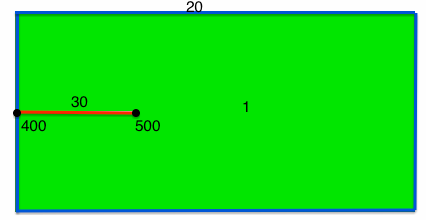
\includegraphics[width=.45\textwidth]{Examples/Surfing/Geometry.png}
\caption{Domain for the Surfing example. The numbers correspond to cubit entities.}
\label{fig:Surfing}
\end{figure}



\section*{Proposed numerical experimentations:}
\begin{enumerate}
\item Check the qualitative fracture behavior in a surfing experiment (crack path, initial length at reactivation, ...).
\item Study the effect of the damage boundary condition along the crack or at the crack tip on the crack propagation. Is activation always progressive?
\item Study the effect of the numerical effective toughness on crack loading at initiation. Can this effect be accounted for \emph{a priori}?
\end{enumerate}

\section{Enforcing Displacement boundary conditions}
Consider the domain from figure~\ref{fig:BC}. Prescribe the vertical component of the displacement along the left edge, while the lower edges are clamped. See how if the damage is left free on the lower edge, the surface energy of a boundary crack is mis-calculated.
\begin{figure}[H]
\centering

\includegraphics[width=.45\textwidth]{Examples/BC/Geometry.png}
\caption{Domain for the Surfing example. The numbers correspond to cubit entities.}
\label{fig:BC}
\end{figure}



\section{Cooling}
This problem replicates the thermal shock experiment studied in depth in~\cite{Sicsic-Marigo-2013a,Bourdin-Marigo-EtAl-2014a}. A rectangular domain held at initial temperature $T_0$ is subject to the boundary temperature $T(x,t) = T_0 - \Delta T$ on its boundary. In two dimension, the behavior depends on a single parameter quantifying the intensity of the thermal shock in relation with the material thermo-mechanical properties.

The renormalized material properties for this problem are $E = 3.4\times 10^5 \mathrm{Nmm}^{-2}$, $\nu = .22$, $k = .0424 \mathrm{Nmm}^{-1}$, $\alpha_L = 8\times10^{-6} \mathbf{I}\mathrm{K}^{-1}$, $\ell = .05\mathrm{mm}$. For a domain of size $50 \mathrm{mm} \times 10 \mathrm{mm}$, assuming a unit thermal conductivity and a temperature contrast of $380\mathrm{K}$, the crack evolution should take place within $1\mathrm{s}$.


Journal and data files are located in  \verb+Examples/Cooling+

\section*{Proposed activities}
\begin{itemize}
\item Approximate a semi-infinite domain by applying a prescribe temperature along the long edge of the domain, and null flux and roller displacement boundary conditions along all other edges. See how distributed damage arises only above above a critical temperature contrast.
\item See how distributed damage evolves into localized damaged areas then into cracks, and how the crack spacing and depth depend on the internal length.
\item Highlight the ``parking'' selection mechanism.
\item Re-run on a full or quarter domain.
\end{itemize}

\section{Bi-layer}
Consider a domain consisting of two layers with a pre-existing crack on the upper layer. Create an inelastic strain by applying a constant temperature field to the layers and applying different elasticity modulii and thermal expansion coefficients to each layer.

\section*{Proposed numerical experimentations:}
By varying the displacement boundary condition on the lower edge (roller of stress free), and relative mechanical properties in the layers, multiple fracture behaviors can be exhibited: nucleation of periodic crack in the upper later as in the cooling problem, a single crack penetrating in the lower layer before branching, a crack propagating along the interface,...
Alternatively, the python script from the surfing example could be used to apply a pre-computed inelastic strain.


\bibliography{vDef}
\end{document}  